\documentclass[t]{beamer} \usepackage[english]{babel} \usepackage[utf8]{inputenc} \usetheme{Frankfurt} %{{{
\usefonttheme{serif} \usepackage{palatino}
\let\OLDsection\section \renewcommand{\section}[1]{\OLDsection{#1} \subsection{}} % each slide has a bullet even when no subsections used
\usepackage{booktabs,amsmath,amsfonts,graphicx,sidecap,upgreek}
\usepackage{tikz} \tikzstyle{every picture}+=[remember picture] \everymath{\displaystyle}
\usepackage{textpos} 

\beamersetleftmargin{3mm} \beamersetrightmargin{3mm}
\definecolor{myblue}{rgb}{0.10, 0.30, 0.50}
\usecolortheme[named=myblue]{structure}
\setbeamertemplate{navigation symbols}{\color{myblue}\footnotesize\insertframenumber}			% leave only tiny page number at the bottom
\setbeamerfont*{frametitle}{size=\normalsize,series=\bfseries}
%}}}
\hypersetup{
        pdftitle={Metamaterials for the Terahertz Spectral Range},
        pdfauthor={Ing. Filip Dominec},
        pdfsubject={},
        pdfkeywords={}
}

\usepackage[
  language=english,
  %urldate=long,
  style=numeric,
  sorting=none,
  isbn=true,
  doi=false,
  url=true,
  firstinits=true,  % will render all first and middle names as initials.
  abbreviate=false,
  autolang=hyphen,
  backend=biber,
  maxbibnames=3]{biblatex}
\renewbibmacro{in:}{%
  \ifentrytype{article}{}{\printtext{\bibstring{in}\intitlepunct}}}
% Volume number must be typeset in bold
\DeclareFieldFormat[article]{volume}{\textbf{#1}}% volume of a journal

% Pages must not be leaded by any "Pages:" word
\DeclareFieldFormat[article]{pages}{#1}% volume of a journal

% Year must be in paretheses
\DeclareFieldFormat[article]{date}{\mkbibparens{#1}}

% Remove quotation of title
\DeclareFieldFormat
  [article,inbook,incollection,inproceedings,patent,thesis,unpublished]
  {title}{#1\isdot}

% Comma NOT before BUT after journal volume
    \renewbibmacro*{volume+number+eid}{%
      %\setunit*{\addcomma\space}% NEW
      \printfield{volume}%
    %  \setunit*{\adddot}% DELETED
      %\setunit*{\addcomma\space}% NEW
      %\printfield{number}%
      %\setunit{\addcomma\space}%
      \printfield{eid}
}





% Comma before date; date not in parentheses
\renewbibmacro*{issue+date}{%
  %\setunit*{\addcomma\space}% 	 DELETED comma
%  \printtext[parens]{% DELETED
    \iffieldundef{issue}
      {\usebibmacro{date}}
      {\printfield{issue}%
       %\setunit*{\addspace}%
%       \usebibmacro{date}}}% DELETED
       \usebibmacro{date}}% NEW
  \newunit}

% Issue/date macros removed after journal number
\renewbibmacro*{journal+issuetitle}{%
  \usebibmacro{journal}%
  \setunit*{\addspace}%	 RETURNED HERE, avoid dot or comma after journal name
  \iffieldundef{series}
    {}
    {\newunit
     \printfield{series}%
     %\setunit{\addspace}}%	 DELETED comma
	}
  \usebibmacro{volume+number+eid}%
%  \setunit{\addspace}% DELETED
  %\usebibmacro{issue+date}% DELETED
%  \setunit{\addcolon\space}% DELETED
%  \usebibmacro{issue}% DELETED
  \newunit}

% "In:" removed for articles; issue/date macros added after note+pages macro
\DeclareBibliographyDriver{article}{%
  \usebibmacro{bibindex}%
  \usebibmacro{begentry}%
  \usebibmacro{author/translator+others}%
  \setunit{\labelnamepunct}\newblock
  \usebibmacro{title}%
  \newunit
  \printlist{language}%
  \newunit\newblock
  \usebibmacro{byauthor}%
  \newunit\newblock
  \usebibmacro{bytranslator+others}%
  \newunit\newblock
  \printfield{version}%
  \newunit\newblock
%  \usebibmacro{in:}% DELETED
  \usebibmacro{journal+issuetitle}%
  \newunit
  \usebibmacro{byeditor+others}%
  \newunit
  \usebibmacro{note+pages}%
  \usebibmacro{pageref}% MOVED HERE
  \setunit{\addspace}% NEW
  \usebibmacro{issue+date}% NEW
  \setunit{\addcolon\space}% NEW
  \usebibmacro{issue}% NEW
  \newunit\newblock
  \iftoggle{bbx:isbn}
    {\printfield{issn}}
    {}%
  \newunit\newblock
  \usebibmacro{doi+eprint+url}%
  \newunit\newblock
  \usebibmacro{addendum+pubstate}%
  \setunit{\bibpagerefpunct}\newblock
  %\usebibmacro{pageref}%
  \usebibmacro{finentry}}

\addbibresource{../fdphd.bib}



\title[THz MMs]{Metamaterials for the Terahertz Spectral Range}
\author{Ing. Filip Dominec} 
\institute{Advisor: Dr. Mgr. Filip Kadlec (Fyzikální ústav AVČR)\\ Consultant: doc. Dr. Ing. Ivan Richter (FJFI ČVUT)\vspace{2mm}\\ Opponents: doc. Ing. Lukáš Jelínek, Ph.D.,\\
and doc. Dr. Mgr. Kamil Postava (VŠB-TU Ostrava) } 
\date{Ph. D. Dissertation Defence\\ 13$^{\mathrm{th}}$ December 2016}

\newcommand{\again}{again}
\newcommand{\E}{\mathbf{E}}
\newcommand{\D}{\mathbf{D}}
\newcommand{\B}{\mathbf{B}}
\newcommand{\HH}{\mathbf{H}}
\newcommand{\Dsd}{{\mathbf{D}^\text{LL}}}
\newcommand{\HHsd}{{\mathbf{H}^\text{LL}}}

\newcommand{\epsrl}{\varepsilon_r} 		%% local
\newcommand{\murl}{\mu_r}			
\newcommand{\epsrn}{\varepsilon_r}		%% nonlocal symmetric - uses the same notation as for local, only arguments are (omega,k)
\newcommand{\murn}{\mu_r}
\newcommand{\epsLL}{\varepsilon_r^\text{LL}}	%% nonlocal Landau-Lifshitz
\newcommand{\muLL}{\mu_r^\text{LL}}


\newcommand{\Neff}{N_{\text{eff} }}		%% effective
\newcommand{\Zeff}{Z_{\text{eff} }}
\newcommand{\eeff}{\varepsilon_{\text{eff} }}
\newcommand{\meff}{\mu_{\text{eff} }}

\newcommand{\ii}{{\mathrm i}}
\newcommand{\rr}{{\mathbf{r}}}
\newcommand{\brho}{\boldsymbol{\rho}}

\newcommand{\kk}{{\mathbf{k}}}
\newcommand{\KK}{{\mathbf{K}}}
\newcommand{\TT}{\perp_{\mathbf{k}}}
%\newcommand{\TT}{\small{\frac{\kk\times\kk\times}{-k^2}}}
\newcommand{\epsr}{{\varepsilon_r}}
\newcommand{\vg}{{\mathbf{v_g}}}

\newcommand{\ava}{{\mathbf{a_1}}}
\newcommand{\avb}{{\mathbf{a_2}}}
\newcommand{\avc}{{\mathbf{a_3}}}
\newcommand{\avabc}{{\mathbf{a_{1,2,3}}}}


\newcommand{\add}[1]{\color{blue}#1\color{black}{}}
\newcommand{\rmv}[1]{\color{grey}\ensuremath{\vdash}#1\ensuremath{\dashv}\color{black}{}}
\newcommand{\mdf}[1]{{\color{red}#1}}
\newcommand{\todo}[1]{{\color{red}\textbf{\texttt{TODO: #1}}}}
\newcommand{\coloruse}{\marginpar{\scriptsize
\add%
{added}\\ \mdf%
{modified}\\ \rmv%
{deleted} }}



\begin{document}

\section{Introduction}
\begin{frame}		%{{{ Titulní stránka
	\titlepage
\end{frame}		%}}}
%\begin{frame}[plain]{\tiny{\vspace{-1em}A text\vspace{-.5em}}}	%{{{

%\begin{array}
%\nabla \cdot  \D = 0,\\
%\nabla \cdot  \B = 0,\\
%\nabla \times \E = -\frac{\partial \B} {\partial t},\\
%\nabla \times \HH =  \frac{\partial \D} {\partial t},
%\end{array}

\begin{frame}{Thesis goals in short} 		%{{{
	\begin{enumerate}
		 \item{Elaborate an accessible theoretical background describing the \textbf{electrodynamics of periodic structures}} 
		 \item{Emphasize the importance of taking the \textbf{nonlocal medium response} into account} 
		 \item{Examine, in particular, structures lying \textbf{at the boundary} between the metamaterial and photonic crystal paradigms} 
		 \item{Experimentally validate part of the numerical results, and \textbf{compose an overview} of periodic structures behaviour} 
		 \item{Ensure that all developed simulation scripts are \textbf{published online}} 
	\end{enumerate}
\end{frame} 		%}}}

\begin{frame}{What are metamaterials?} 		%{{{
\begin{exampleblock}{Proposed definition of a metamaterial}
A metamaterial is any inhomogeneous structure with behaviour determined more by its shape than by constituent materials, that we attempt to describe as a homogeneous one
\end{exampleblock}

More usually, metamaterials are defined as periodic structures artificially designed to achieve some values of \textit{effective parameters} that are not found in natural materials.

\vfill
Large part of metamaterial research is aimed at achieving \textit{negative effective index of refraction} $\Neff'<0$, which is expected to occur if simultaneously the effective permittivity $\eeff' <0$ and permeability $\meff'<0$ are negative.
%Then, the task of finding the effective parameters (homogenisation) is more fundamental than just a means of characterisation: It \textit{defines} that the structure \textit{is} a metamaterial.
\end{frame} 		%}}}

\begin{frame}[plain]{\tiny{\vspace{-1em}{Early metamaterials -- artificial dielectrics}\vspace{-.5em}}} %{{{
\includegraphics[width=\textwidth]{../img/patents/mm_patents.pdf} 

%\textbf{(a)} sheets containing cut wires of alternating orientation and resonant frequency, enabling one to manipulate the microwave polarisation, \textbf{(b)} cross-section through a lightweight lens of 3 m diameter designed for 50-500 MHz radio waves, made of partially metallized plastic layers, \textbf{(c)} artificial dielectric made of non-resonant cut wires arranged into a nearly isotropic 3-D lattice. 
\vfill
\tiny{J. A. F. Wickersham. Artificial dielectric polarizer. US Patent 2,921,312. 1960. URL : http://www.google.com/patents/US2921312.\\
D. L. Anderson. Artificial dielectric lens structure. US Patent 3,329,958. 1967. URL : http://google.ru/patents/US3329958.\\
P. W. Hannan. Artificial dielectric using interspersed rods. US Patent 3,254,345. 1966. URL : http://www.google.com.py/patents/US3254345.}
\end{frame}%}}}


\begin{frame}{Early photonic crystals} 		%{{{
\vspace{-.5em}
Photonic crystals (PhC) are periodic structures aimed at engineering the photonic band gap and density of states. 
Their effective parameters are usually not determined.

%\vspace{.5em}
%Probably the first PhC, proposed by E. Yablonovitch in 1987, was manually drilled into a block of acrylic glass.

\vfill
\includegraphics[width=\textwidth]{../img/patents/phc_patents.pdf} 
\vfill

\tiny{E. Yablonovitch. Inhibited Spontaneous Emission in Solid-State Physics and Electronics. Phys. Rev. Lett. 58, 2059–2062 20(1987).\\
K. Ho, C. Chan, and C. Soukoulis. Periodic dielectric structure for production of photonic band gap and devices incorporating the same. US Patent 5,335,240. 1994.  URL : https://www.google.com.ar/patents/US5335240.\\
W. Sweatt and T. Christenson. Method for the fabrication of three-dimensional microstructures by deep X-ray lithography. US Patent 6,875,544. 2005. URL : https://www.google.com.ar/patents/US6875544.  }
\end{frame} 		%}}}

\begin{frame}{2000's: Merging of MM and PhC paradigms?} 		%{{{
Two paradigms of \textit{metamaterials} (MM), which were earlier denoted as \textit{artificial dielectrics}, and \textit{photonic crystals} (PhC) developed separately over few decades.

\begin{exampleblock}{Waves in periodic structures vs. in natural media}
\centering \begin{tabular}{lcccr}
Light in MMs    &$\leftrightarrow$  &$\lambda \gg a$ &$\leftrightarrow$ 	& Light in a crystal         	\\
Light in PhCs   &$\leftrightarrow$  &$\lambda \sim a$ &$\leftrightarrow$ 	& Electron wave in a crystal 	\\
\end{tabular}
\end{exampleblock}

However, as the metamaterial research approaches the optical frequencies,  the $\lambda \gg a$ limit can not be held.
%(Note that this is determined by available materials, not a mere issue of today's technology)
\vspace{.5em}
\end{frame} 		%}}}

\begin{frame}{The metamaterial assumption $\lambda_0 \gg a$ is unsustainable}	%{{{
	{\vspace{-.1em}\hfill \ldots for majority of realistic NIR/optical metamaterials}

\vspace{-1em}
\begin{table}[ht]   \caption{Short survey for the ratio of free-space wavelength $\lambda_0$ to the unit-cell size (parallel and perpendicular to $\kk$) in selected publications}  \label{tb_} \centering 
\begin{tabular}{lrrrr}
\toprule
	Source		 & $\lambda_0$ (nm)	& $\lambda_0/a_{||}$  & $\lambda_0/a_{\perp}$ & type \\
\hline
Šindler et al. 2016  & 350000		&  6--10	& 6--10 & Mie \\
Zhang et al. 2005    & 1300			&  7        & \textbf{2.2}  & SRR \\
Dolling et al. 2007  & 780			&  8		& \textbf{2.6}  & fishnet \\
Gong et al. 2014     & 565			&  8		& \textbf{2.4}  & fishnet \\
Aslam et al. 2012    & 510			&  14		& \textbf{2.1}  & fishnet \\
Xu et al. 2013	     & 365		    & \textbf{2.4}		& --	& 2-D layers \\
\bottomrule
\end{tabular} \end{table}

\vspace{.5em}

We must carefully review all approaches to MMs that assume that the unit cells $a$ are \textit{just small}; in practice, they are not.
	\vfill
	\tiny{	
Šindler, M., et al., Optics Express, 24(16), 18340-18345, (2016);  Zhang, S. et al., Phys. Rev. Lett., 94(3), 037402 (2005).\\
Dolling et al. Opt. Lett. 32, 53–55 (2007); Gong, B., et al.,. Sci. Rep., 4 (2014).\\
Aslam, M. I., and Güney, D. Ö. JOSA B, 29(10), 2839-2847 (2012).; Xu, T., et al., Nature, 497(7450), 470-474  (2013).}
\end{frame} 		%}}}


\section{Dielectric-rod array}
\begin{frame}{Dielectric rod array}	%{{{

\vspace{-.6em}
\ldots has been investigated first as a photonic crystal with a photonic band gap, and since 2000s also as a metamaterial with $\Neff'<0$. 
\begin{tiny}\end{tiny}

\vspace{.3em}

\hfill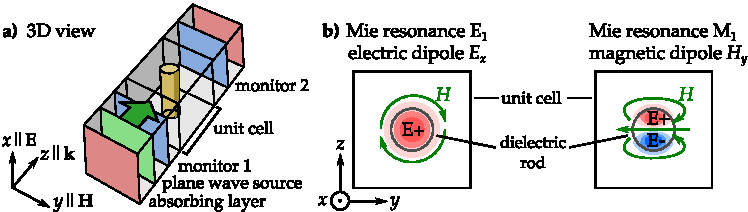
\includegraphics[width=1\textwidth]{../img/ERods_1st_and_2nd_Mie_resonance_sketch.pdf}\hfill\;
\vspace{.3em}

%The first Mie resonance has an electric dipole moment only, while the second one has a magnetic dipole moment instead. 
\textbf{(a)} Simulation layout for computation of $\Neff, \Zeff, \eeff$ and $\meff$ using the \textit{scattering-parameters} method. Cells are periodic in the \textbf{x} and \textbf{y} directions. \\
\textbf{(b)} Cross-sections through the \textbf{y}-\textbf{z} plane showing two resonant modes. The dielectric permittivity at $f$ = 1 THz was 89.5 + 0.23i, corresponding to polycrystalline titanium dioxide.

\vfill
\begin{tiny}W. B. Weir. Proc. IEEE 62, 33–36 (1974); A. Nicolson and G. Ross. Instrum. Meas., IEEE Transactions on, 19, 377–382 (1970).\end{tiny}
\end{frame} 		%}}}

\begin{frame}[plain]{}	%{{{
\hspace{6mm} \includegraphics[height=.97\paperheight]{../img/ERods_eps100_single_a120_FDTD.pdf}
\end{frame} 		%}}}

\begin{frame}[plain]{}	%{{{
\hspace{6mm} \includegraphics[width=1.12\paperheight]{../img/ERods_eps100_double_a100a080_FDTD.pdf}
\end{frame} 		%}}}

\begin{frame}{Color coding of refractive index}	%{{{
\includegraphics[width=1.\framewidth]{../img/ERods_sketch_of_separate_spectra_to_continuous_scan.pdf}
\end{frame} 		%}}}

\begin{frame}{Spacing scan: $\Neff', \Neff''$  for $\pmb\rho=10\;\upmu$m, $\pmb\varepsilon_r=100$}	%{{{
Real ($\Neff'$, left panel) and imaginary ($\Neff''$, right panel) parts of refractive indices 
% TODO rm Rods_eps100_spacingscan_Nim.pdf% TODO rm Rods_eps100_spacingscan_Nim.pdf

{\centering
\mbox{\includegraphics[width=62mm]{../img/ERods_eps100_spacingscan_Nre.pdf}\includegraphics[width=62mm]{../img/ERods_eps100_spacingscan_Nim.pdf}} \vspace{-5mm} }
\end{frame} 		%}}}

\begin{frame}{Dielectric rod array -- sketch of spacing scan}	%{{{

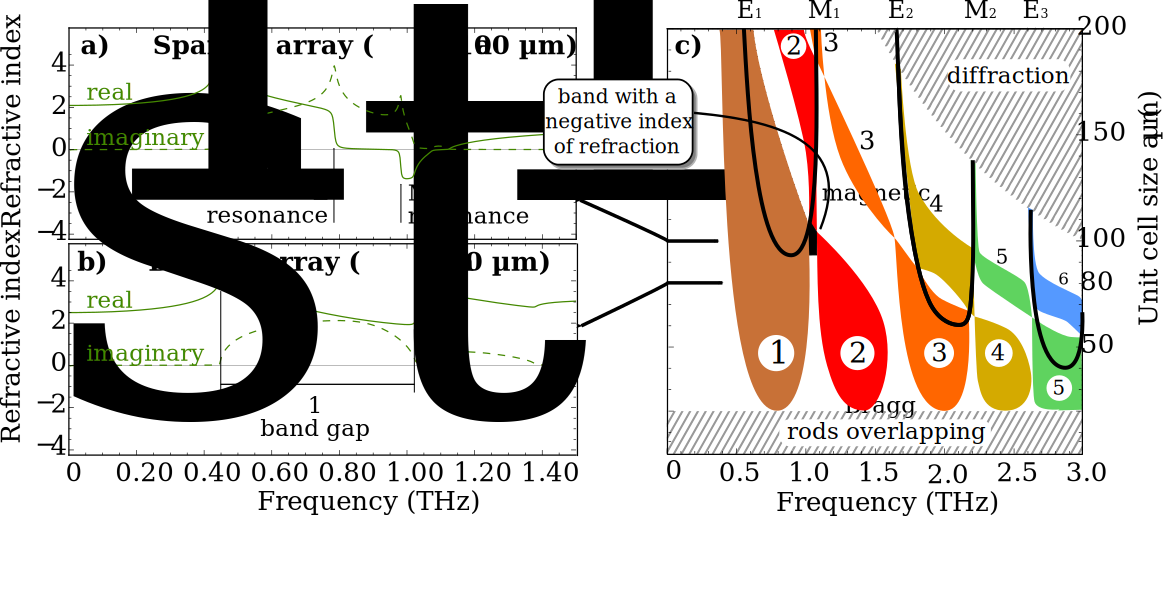
\includegraphics[width=\textwidth]{../img/ERods_forSeefeld_sparserN_denserN_DrawnBands.pdf}

\vfill
\tiny{F. Dominec et al. Transition between metamaterial and photonic-crystal behavior in arrays of dielectric rods. Opt. Express 22, 30492--30503 (2014).\\
M. V. Rybin et al. Phase diagram for the transition from photonic crystals to dielectric metamaterials. arXiv:1507.08901 (2015).}
\end{frame} 		%}}}

\section{Spatial dispersion}
\begin{frame}{Nonlocal response}%{{{
The trouble with using $\eeff(\omega)$ and $\meff(\omega)$ is that they only describe the local response. \vspace{.5em}

The medium may be \textit{nonlocal}, i.e., elecric field in point $\rr$ makes it develop polarisation also in surrounding points $\rr\neq\rr'$.
	
\begin{exampleblock}{Waves in periodic structures vs. in natural media II.}
\centering \begin{tabular}{lcccr}
Light in MMs    &$\leftrightarrow$  &$\lambda \gg a$ &$\leftrightarrow$ 	& Light in a crystal         	\\
Light in PhCs   &$\leftrightarrow$  &$\lambda \sim a$ &$\leftrightarrow$ 	& Electron wave in a crystal 	\\
	\textbf{Previous example}  &$\leftrightarrow$  &$\mathbf{\pmb{\lambda\lesssim a}}$ &$\leftrightarrow$ 	& \textbf{Nonlocal medium!}\\
\end{tabular}
\end{exampleblock}

For a harmonic wave, nonlocality translates into \textit{spatial dispersion}, and the effective parameters explicitly depend on the wave vector $\kk$: 
$$\epsrl(\omega), \murl(\omega) \rightarrow  \epsrn(\omega,\kk), \murn(\omega,\kk)$$
\end{frame} %}}}

\begin{frame}{Current-driven homogenization}%{{{
The customary approach involved selecting a frequency, measuring the scattering parameters (reflectance and transmittance) and computing the allowed wavenumbers.
 \vspace{.2em}

\begin{columns}[T] % align columns
	\begin{column}{.5\textwidth}
		\hfill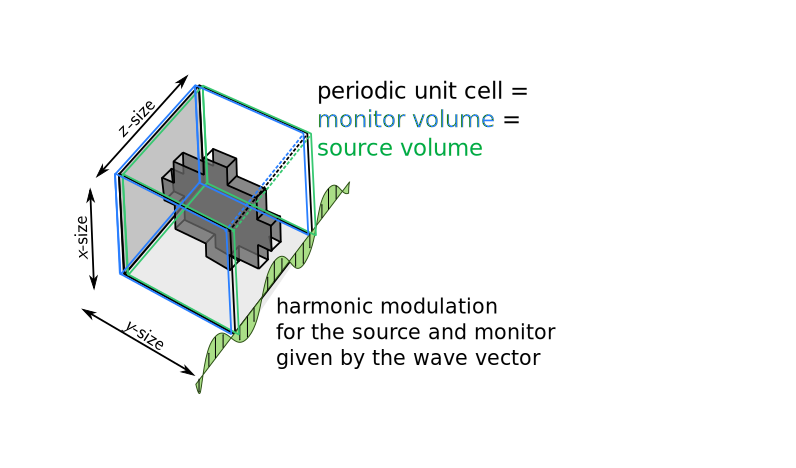
\includegraphics[width=.9\textwidth]{../img/cdh_geometry.pdf}
	\end{column}
	\begin{column}{.5\textwidth}
	\vspace{3mm}
	\noindent Instead, in the \textit{current-driven homogenization}, the volumetric current source imparts a desired wavevector $\KK$ to the whole unit cell, and looks for all corresponding resonance frequencies.
\end{column}%
\end{columns}
 \vspace{.2em}


\vfill 
\begin{tiny}
M. G. Silveirinha. Metamaterial homogenization approach with application to the characterization of microstructured composites with negative parameters. Phys. Rev. B 75, 115104 (2007). \\
C. Fietz and G. Shvets. Current-driven metamaterial homogenization. Physica B 405, 2930–2934 (2010).
\end{tiny}
\end{frame} 		%}}}

\begin{frame}[plain]{}%{{{
\begin{columns}[T] % align columns
	\begin{column}{.55\textwidth}
	\vspace{3mm}
	\noindent Testing current-driven homogenization (CDH) on the rod array with $a=$ 100 $\upmu$m, $\rho=10\;\upmu$m, $\varepsilon_r=100$ 	$\rightarrow$
	\vspace{3mm}

	\noindent Bubbles are computed using CDH; the green dispersion curve shows the effective index of refraction from the scattering-parameters method as $$K = \frac{2\pi \Neff' \;f}{c}.$$ Dashed part denotes negative values of $\Neff$
	\vspace{3mm}
	\begin{exampleblock}{Result}
	\noindent This confirms that the use of scattering parameter method was appropriate for this rod array
	\end{exampleblock}

	\end{column}%
	\begin{column}{.45\textwidth}
		\vspace{-1mm}\includegraphics[height=\paperheight]{../img-cdh-new/CDH_RodArray.pdf} 
	\end{column}
\end{columns}
\end{frame} 		%}}}

\section{Combined SRR}
\begin{frame}{Electro-magnetic split-ring resonator}%{{{
%\noindent We will examine the dispersion of a metamaterial composed of a combined electro-magnetic split-ring resonator:

\hfill\includegraphics[width=.85\textwidth]{../img-cdh-new/emSRR_snapshot.pdf} \hfill\;
\end{frame} %}}}

\begin{frame}{Electro-magnetic split-ring resonances}%{{{
The structure exhibits two resonances; one with a magnetic dipole (left) the second with an electric one (right).

\hfill\includegraphics[height=0.22\textwidth]{../img/drawing_emcSRRpad_resM.pdf}\hfill
\includegraphics[height=0.22\textwidth]{../img/drawing_emcSRRpad_resE2.pdf}\hfill\;

By changing the inner capacitor radius, we can tune the electric resonance frequency.

\vfill
Other parameters will remain constant: capacitor splitting := 6 $\upmu$m, outer ring radius := 45 $\upmu$m, conductor cross-section := 10$\times$10 $\upmu$m and unit cell size := 100$\times$100$\times$100 $\upmu$m.
\end{frame} %}}}


\begin{frame}[plain]{}%{{{
\begin{columns}[T] % align columns%{{{
	\begin{column}{.55\textwidth}
	\vspace{3mm}
	\noindent Current-driven homogenization (CDH) of an electro-magnetic split-ring resonator 
	\begin{exampleblock}\hfill inner capacitor radius of $\pmb\rho_c=\pmb{6}\;\upmu$m $\rightarrow$\end{exampleblock}
	\vspace{3mm}

	\noindent Bubbles are computed using CDH; the green dispersion curve comes from the scattering-parameters method. Note that $$K = \frac{2\pi n f}{c}$$
	\vspace{12mm}

	\small{capacitor splitting = 6 $\upmu$m,\\ outer ring radius = 45 $\upmu$m,\\ conductor cross-section = 10$\times$10 $\upmu$m\\ unit cell size = 100$\times$100$\times$100 $\upmu$m}
	%\begin{exampleblock}{Result} ## TODO 
	%\noindent This confirms that the use of scattering parameter method was appropriate  for this structure
	%\end{exampleblock}

	\end{column}%
	\begin{column}{.45\textwidth}%}}}
		\vspace{-1mm}\includegraphics[height=\paperheight]{../img-cdh-new/CDH_SRRArray_06.pdf} 
	\end{column}
\end{columns}
\end{frame} 		%}}}
\begin{frame}[plain]{}%{{{
\begin{columns}[T] % align columns%{{{
	\begin{column}{.55\textwidth}
	\vspace{3mm}
	\noindent Current-driven homogenization (CDH) of an electro-magnetic split-ring resonator 
	\begin{exampleblock}\hfill inner capacitor radius of $\pmb\rho_c=\pmb{7}\;\upmu$m $\rightarrow$\end{exampleblock}
	\vspace{3mm}

	\noindent Bubbles are computed using CDH; the green dispersion curve comes from the scattering-parameters method. Note that $$K = \frac{2\pi n f}{c}$$
	\vspace{12mm}

	\small{capacitor splitting = 6 $\upmu$m,\\ outer ring radius = 45 $\upmu$m,\\ conductor cross-section = 10$\times$10 $\upmu$m\\ unit cell size = 100$\times$100$\times$100 $\upmu$m}
	\vspace{5mm}
	%\begin{exampleblock}{Result} ## TODO 
	%\noindent This confirms that the use of scattering parameter method was appropriate  for this structure
	%\end{exampleblock}

	\end{column}%
	\begin{column}{.45\textwidth}%}}}
		\vspace{-1mm}\includegraphics[height=\paperheight]{../img-cdh-new/CDH_SRRArray_07.pdf} 
	\end{column}
\end{columns}
\end{frame} 		%}}}
\begin{frame}[plain]{}%{{{
\begin{columns}[T] % align columns%{{{
	\begin{column}{.55\textwidth}
	\vspace{3mm}
	\noindent Current-driven homogenization (CDH) of an electro-magnetic split-ring resonator 
	\begin{exampleblock}\hfill inner capacitor radius of $\pmb\rho_c=\pmb{8}\;\upmu$m $\rightarrow$\end{exampleblock}
	\vspace{3mm}

	\noindent Bubbles are computed using CDH; the green dispersion curve comes from the scattering-parameters method. Note that $$K = \frac{2\pi n f}{c}$$
	\vspace{12mm}

	\small{capacitor splitting = 6 $\upmu$m,\\ outer ring radius = 45 $\upmu$m,\\ conductor cross-section = 10$\times$10 $\upmu$m\\ unit cell size = 100$\times$100$\times$100 $\upmu$m}
	\vspace{5mm}
	%\begin{exampleblock}{Result} ## TODO 
	%\noindent This confirms that the use of scattering parameter method was appropriate  for this structure
	%\end{exampleblock}

	\end{column}%
	\begin{column}{.45\textwidth}%}}}
		\vspace{-1mm}\includegraphics[height=\paperheight]{../img-cdh-new/CDH_SRRArray_08.pdf} 
	\end{column}
\end{columns}
\end{frame} 		%}}}
\begin{frame}[plain]{}%{{{
\begin{columns}[T] % align columns%{{{
	\begin{column}{.55\textwidth}
	\vspace{3mm}
	\noindent Current-driven homogenization (CDH) of an electro-magnetic split-ring resonator 
	\begin{exampleblock}\hfill inner capacitor radius of $\pmb\rho_c=\pmb{9}\;\upmu$m $\rightarrow$\end{exampleblock}
	\vspace{3mm}

	\noindent Bubbles are computed using CDH; the green dispersion curve comes from the scattering-parameters method. Note that $$K = \frac{2\pi n f}{c}$$
	\vspace{12mm}

	\small{capacitor splitting = 6 $\upmu$m,\\ outer ring radius = 45 $\upmu$m,\\ conductor cross-section = 10$\times$10 $\upmu$m\\ unit cell size = 100$\times$100$\times$100 $\upmu$m}
	\vspace{5mm}
	%\begin{exampleblock}{Result} ## TODO 
	%\noindent This confirms that the use of scattering parameter method was appropriate  for this structure
	%\end{exampleblock}

	\end{column}%
	\begin{column}{.45\textwidth}%}}}
		\vspace{-1mm}\includegraphics[height=\paperheight]{../img-cdh-new/CDH_SRRArray_09.pdf} 
	\end{column}
\end{columns}
\end{frame} 		%}}}
\begin{frame}[plain]{}%{{{
\begin{columns}[T] % align columns%{{{
	\begin{column}{.55\textwidth}
	\vspace{3mm}
	\noindent Current-driven homogenization (CDH) of an electro-magnetic split-ring resonator 
	\begin{exampleblock}\hfill inner capacitor radius of $\pmb\rho_c=\pmb{10}\;\upmu$m $\rightarrow$\end{exampleblock}
	\vspace{3mm}

	\noindent Bubbles are computed using CDH; the green dispersion curve comes from the scattering-parameters method. Note that $$K = \frac{2\pi n f}{c}$$
	\vspace{12mm}

	\small{capacitor splitting = 6 $\upmu$m,\\ outer ring radius = 45 $\upmu$m,\\ conductor cross-section = 10$\times$10 $\upmu$m\\ unit cell size = 100$\times$100$\times$100 $\upmu$m}
	\vspace{5mm}
	%\begin{exampleblock}{Result} ## TODO 
	%\noindent This confirms that the use of scattering parameter method was appropriate  for this structure
	%\end{exampleblock}

	\end{column}%
	\begin{column}{.45\textwidth}%}}}
		\vspace{-1mm}\includegraphics[height=\paperheight]{../img-cdh-new/CDH_SRRArray_10.pdf} 
	\end{column}
\end{columns}
\end{frame} 		%}}}
\begin{frame}[plain]{}%{{{
\begin{columns}[T] % align columns%{{{
	\begin{column}{.55\textwidth}
	\vspace{3mm}
	\noindent Current-driven homogenization (CDH) of an electro-magnetic split-ring resonator 
	\begin{exampleblock}\hfill inner capacitor radius of $\pmb\rho_c=\pmb{11}\;\upmu$m $\rightarrow$\end{exampleblock}
	\vspace{3mm}

	\noindent Bubbles are computed using CDH; the green dispersion curve comes from the scattering-parameters method. Note that $$K = \frac{2\pi n f}{c}$$
	\vspace{12mm}

	\small{capacitor splitting = 6 $\upmu$m,\\ outer ring radius = 45 $\upmu$m,\\ conductor cross-section = 10$\times$10 $\upmu$m\\ unit cell size = 100$\times$100$\times$100 $\upmu$m}
	\vspace{5mm}
	%\begin{exampleblock}{Result} ## TODO 
	%\noindent This confirms that the use of scattering parameter method was appropriate  for this structure
	%\end{exampleblock}

	\end{column}%
	\begin{column}{.45\textwidth}%}}}
		\vspace{-1mm}\includegraphics[height=\paperheight]{../img-cdh-new/CDH_SRRArray_11.pdf} 
	\end{column}
\end{columns}
\end{frame} 		%}}}
\begin{frame}[plain]{}%{{{
\begin{columns}[T] % align columns%{{{
	\begin{column}{.55\textwidth}
	\vspace{3mm}
	\noindent Current-driven homogenization (CDH) of an electro-magnetic split-ring resonator 
	\begin{exampleblock}\hfill inner capacitor radius of $\pmb\rho_c=\pmb{12}\;\upmu$m $\rightarrow$\end{exampleblock}
	\vspace{3mm}

	\noindent Bubbles are computed using CDH; the green dispersion curve comes from the scattering-parameters method. Note that $$K = \frac{2\pi n f}{c}$$
	\vspace{12mm}

	\small{capacitor splitting = 6 $\upmu$m,\\ outer ring radius = 45 $\upmu$m,\\ conductor cross-section = 10$\times$10 $\upmu$m\\ unit cell size = 100$\times$100$\times$100 $\upmu$m}
	\vspace{5mm}
	%\begin{exampleblock}{Result} ## TODO 
	%\noindent This confirms that the use of scattering parameter method was appropriate  for this structure
	%\end{exampleblock}

	\end{column}%
	\begin{column}{.45\textwidth}%}}}
		\vspace{-1mm}\includegraphics[height=\paperheight]{../img-cdh-new/CDH_SRRArray_12.pdf} 
	\end{column}
\end{columns}
\end{frame} 		%}}}
\begin{frame}[plain]{}%{{{
\begin{columns}[T] % align columns%{{{
	\begin{column}{.55\textwidth}
	\vspace{3mm}
	\noindent Current-driven homogenization (CDH) of an electro-magnetic split-ring resonator 
	\begin{exampleblock}\hfill inner capacitor radius of $\pmb\rho_c=\pmb{13}\;\upmu$m $\rightarrow$\end{exampleblock}
	\vspace{3mm}

	\noindent Bubbles are computed using CDH; the green dispersion curve comes from the scattering-parameters method. Note that $$K = \frac{2\pi n f}{c}$$
	\vspace{12mm}

	\small{capacitor splitting = 6 $\upmu$m,\\ outer ring radius = 45 $\upmu$m,\\ conductor cross-section = 10$\times$10 $\upmu$m\\ unit cell size = 100$\times$100$\times$100 $\upmu$m}
	\vspace{5mm}
	%\begin{exampleblock}{Result} ## TODO 
	%\noindent This confirms that the use of scattering parameter method was appropriate  for this structure
	%\end{exampleblock}

	\end{column}%
	\begin{column}{.45\textwidth}%}}}
		\vspace{-1mm}\includegraphics[height=\paperheight]{../img-cdh-new/CDH_SRRArray_13.pdf} 
	\end{column}
\end{columns}
\end{frame} 		%}}}
\begin{frame}[plain]{}%{{{
\begin{columns}[T] % align columns%{{{
	\begin{column}{.55\textwidth}
	\vspace{3mm}
	\noindent Current-driven homogenization (CDH) of an electro-magnetic split-ring resonator 
	\begin{exampleblock}\hfill inner capacitor radius of $\pmb\rho_c=\pmb{14}\;\upmu$m $\rightarrow$\end{exampleblock}
	\vspace{3mm}

	\noindent Bubbles are computed using CDH; the green dispersion curve comes from the scattering-parameters method. Note that $$K = \frac{2\pi n f}{c}$$
	\vspace{12mm}

	\small{capacitor splitting = 6 $\upmu$m,\\ outer ring radius = 45 $\upmu$m,\\ conductor cross-section = 10$\times$10 $\upmu$m\\ unit cell size = 100$\times$100$\times$100 $\upmu$m}
	\vspace{5mm}
	%\begin{exampleblock}{Result} ## TODO 
	%\noindent This confirms that the use of scattering parameter method was appropriate  for this structure
	%\end{exampleblock}

	\end{column}%
	\begin{column}{.45\textwidth}%}}}
		\vspace{-1mm}\includegraphics[height=\paperheight]{../img-cdh-new/CDH_SRRArray_14.pdf} 
	\end{column}
\end{columns}
\end{frame} 		%}}}
\begin{frame}[plain]{}%{{{
\begin{columns}[T] % align columns%{{{
	\begin{column}{.55\textwidth}
	\vspace{3mm}
	\noindent Current-driven homogenization (CDH) of an electro-magnetic split-ring resonator 
	\begin{exampleblock}\hfill inner capacitor radius of $\pmb\rho_c=\pmb{15}\;\upmu$m $\rightarrow$\end{exampleblock}
	\vspace{3mm}

	\noindent Bubbles are computed using CDH; the green dispersion curve comes from the scattering-parameters method. Note that $$K = \frac{2\pi n f}{c}$$
	\vspace{12mm}

	\small{capacitor splitting = 6 $\upmu$m,\\ outer ring radius = 45 $\upmu$m,\\ conductor cross-section = 10$\times$10 $\upmu$m\\ unit cell size = 100$\times$100$\times$100 $\upmu$m}
	\vspace{5mm}
	%\begin{exampleblock}{Result} ## TODO 
	%\noindent This confirms that the use of scattering parameter method was appropriate  for this structure
	%\end{exampleblock}

	\end{column}%
	\begin{column}{.45\textwidth}%}}}
		\vspace{-1mm}\includegraphics[height=\paperheight]{../img-cdh-new/CDH_SRRArray_15.pdf} 
	\end{column}
\end{columns}
\end{frame} 		%}}}
% \begin{frame}[plain]{}%{{{
% \begin{columns}[T] % align columns%{{{
% 	\begin{column}{.55\textwidth}
% 	\vspace{3mm}
% 	\noindent Current-driven homogenization (CDH) of an electro-magnetic split-ring resonator 
	%\begin{exampleblock}\hfill inner capacitor radius of $\pmb\rho_c=\pmb{16}\;\upmu$m $\rightarrow$\end{exampleblock}
% 	\vspace{3mm}
% 
% 	\noindent Bubbles are computed using CDH; the green dispersion curve comes from the scattering-parameters method. Note that $$K = \frac{2\pi n f}{c}$$
% 	\vspace{5mm}
% 	%\begin{exampleblock}{Result} ## TODO 
% 	%\noindent This confirms that the use of scattering parameter method was appropriate  for this structure
% 	%\end{exampleblock}
% 
% 	\end{column}%
% 	\begin{column}{.45\textwidth}%}}}
% 		\vspace{-1mm}\includegraphics[height=\paperheight]{../img-cdh-new/CDH_SRRArray_16.pdf} 
% 	\end{column}
% \end{columns}
% \end{frame} 		%}}}
\begin{frame}[plain]{}%{{{
\begin{columns}[T] % align columns%{{{
	\begin{column}{.55\textwidth}
	\vspace{3mm}
	\noindent Current-driven homogenization (CDH) of an electro-magnetic split-ring resonator 
	\begin{exampleblock}\hfill inner capacitor radius of $\pmb\rho_c=\pmb{17}\;\upmu$m $\rightarrow$\end{exampleblock}
	\vspace{3mm}

	\noindent Bubbles are computed using CDH; the green dispersion curve comes from the scattering-parameters method. Note that $$K = \frac{2\pi n f}{c}$$
	\vspace{12mm}

	\small{capacitor splitting = 6 $\upmu$m,\\ outer ring radius = 45 $\upmu$m,\\ conductor cross-section = 10$\times$10 $\upmu$m\\ unit cell size = 100$\times$100$\times$100 $\upmu$m}
	\vspace{5mm}
	%\begin{exampleblock}{Result} ## TODO 
	%\noindent This confirms that the use of scattering parameter method was appropriate  for this structure
	%\end{exampleblock}

	\end{column}%
	\begin{column}{.45\textwidth}%}}}
		\vspace{-1mm}\includegraphics[height=\paperheight]{../img-cdh-new/CDH_SRRArray_17.pdf} 
	\end{column}
\end{columns}
\end{frame} 		%}}}
\begin{frame}[plain]{}%{{{
\begin{columns}[T] % align columns
	\begin{column}{.55\textwidth}
	\vspace{3mm}
	\noindent Current-driven homogenization (CDH) of an electro-magnetic split-ring resonator 
	\begin{exampleblock}\hfill inner capacitor radius of $\pmb\rho_c=\pmb{18}\;\upmu$m $\rightarrow$\end{exampleblock}
	\vspace{3mm}

	\noindent Bubbles are computed using CDH; the green dispersion curve comes from the scattering-parameters method. Note that $$K = \frac{2\pi n f}{c}$$
	\vspace{12mm}

	\small{capacitor splitting = 6 $\upmu$m,\\ outer ring radius = 45 $\upmu$m,\\ conductor cross-section = 10$\times$10 $\upmu$m\\ unit cell size = 100$\times$100$\times$100 $\upmu$m}
	\vspace{5mm}
	%\begin{exampleblock}{Result} ## TODO 
	%\noindent This confirms that the use of scattering parameter method was appropriate  for this structure
	%\end{exampleblock}

	\end{column}%
	\begin{column}{.45\textwidth}
		\vspace{-1mm}\includegraphics[height=\paperheight]{../img-cdh-new/CDH_SRRArray_18.pdf} 
	\end{column}
\end{columns}
\end{frame} 		%}}}

\section{Conclusions}

% "... the losses (that is, absorption) should be reasonably low. Experimental progress in this direction has been sluggish for metal-based metamaterials, but all-dielectric structures avoid- ing metals may provide a solution in some frequency regimes."

\begin{frame}[plain]{\tiny{\vspace{-1em}{Conclusions}\vspace{-.5em}}}%{{{
\begin{itemize}
		\vspace{-.3em}
	\item In the first part of the thesis I summed up relevant metamaterial theory, including topics that I felt to be underemphasized in the literature. 

		%metamaterials approaching the photonic-crystal regime, spatial dispersion must be always taken into account. If not, one often gets puzzling nonphysical results, particularly in $\eeff(\omega)$ and $\meff(\omega)$, but sometimes also in $\Neff(\omega)$.
		%In particular, I prove that the rod-array MM yields negative index of refraction $\Neff'<0$ only in a very narrow range of parameters, and that 

		 %\item{Examine, in particular, structures lying \textbf{at the boundary} between the metamaterial and photonic crystal paradigms} 
	\item I set up an environment for metamaterial simulation and homogenization, and I applied it to structures at the boundary between \textit{metamaterials} and \textit{photonic crystals}. I observed the customary scattering-parameters method to be more limited than is often perceived, and to fail e.g. when stronger spatial dispersion is present.

		 %\item{Emphasize the importance of taking the \textbf{nonlocal medium response} into account} 
	\item A more reliable homogenization scheme (CDH) enabled me to compute the index of refraction for all structures under study.
		% and the extraction of nonlocal $\varepsilon(\omega,\KK)$ prove much more complex than originally expected, 

		 %\item{Experimentally validate part of the numerical results, and \textbf{compose an overview} of periodic structures behaviour} 
	\item In the thesis, I documented the characteristics of ten basic classes of periodic structures, two of which were presented here.

	\item The simulation environment used is published at \\
	\texttt{https://github.com/FilipDominec/python-meep-utils} 
	\vfill
\end{itemize}

\end{frame} %}}}

\begin{frame}[plain]{\tiny{\vspace{-1em}{Conclusions}\vspace{-.5em}}}%{{{
\begin{itemize}
		 %\item{Elaborate an accessible theoretical background describing the \textbf{electrodynamics of periodic structures}} 
		\vspace{-.3em}
	\item In the first part of the thesis I summed up relevant metamaterial theory, including topics that I felt to be underemphasized in the literature. 

		%metamaterials approaching the photonic-crystal regime, spatial dispersion must be always taken into account. If not, one often gets puzzling nonphysical results, particularly in $\eeff(\omega)$ and $\meff(\omega)$, but sometimes also in $\Neff(\omega)$.
		%In particular, I prove that the rod-array MM yields negative index of refraction $\Neff'<0$ only in a very narrow range of parameters, and that 

		 %\item{Examine, in particular, structures lying \textbf{at the boundary} between the metamaterial and photonic crystal paradigms} 
	\item I set up an environment for metamaterial simulation and homogenization, and I applied it to structures at the boundary between \textit{metamaterials} and \textit{photonic crystals}. I observed the customary scattering-parameters method to be more limited than is often perceived, and to fail e.g. when stronger spatial dispersion is present.

		 %\item{Emphasize the importance of taking the \textbf{nonlocal medium response} into account} 
	\item A more reliable homogenization scheme (CDH) enabled me to compute the index of refraction for all structures under study.
		% and the extraction of nonlocal $\varepsilon(\omega,\KK)$ prove much more complex than originally expected, 

		 %\item{Experimentally validate part of the numerical results, and \textbf{compose an overview} of periodic structures behaviour} 
	\item In the thesis, I documented the characteristics of ten basic classes of periodic structures, two of which were presented here.

	\item The simulation environment used is published at \\
	\texttt{https://github.com/FilipDominec/python-meep-utils} 
	\vfill
	{\hfill \color{myblue} \textbf{Thank you for your attention!} \hfill\,}
\end{itemize}

\end{frame} %}}}


\end{document}


